%versi 2 (8-10-2016)
\chapter{Landasan Teori}
\label{chap:teori}

Pada bab ini dibahas dasar teori yang mendukung berjalannya skripsi ini. Dasar teori yang dibahas yaitu Git, JGit, Selenium WebDriver, dan Apache Commons CLI.

\section{Git}
\label{sec:git} 
Seperti yang telah dijelaskan pada subbab \ref{sec:label}, Git merupakan perangkat lunak \textit{Version Control Systems}. Pada subbab ini, dijelaskan mengenai \textit{Version Control Systems}, cara kerja Git, Git \textit{checkout}, dan operasi-operasi dasar pada Git.   

\subsection{Version Control Systems}
\textit{Version Control Systems} adalah sistem yang merekam perubahan pada \textit{file} atau sekumpulan \textit{file} dari waktu ke waktu\cite{chacon2014pro}.\textit{Version Control Systems} biasanya digunakan  untuk merekam file yang berisi \textit{source code program}, tetapi pada kenyataannya \textit{Version Control Systems} dapat merekam hampir semua jenis file dalam komputer. Terdapat tiga jenis \textit{Version Control Systems}, yaitu: \textit{local Version Control Systems}, \textit{centralized Version Control Systems}, dan \textit{distributed Version Control Systems}.

\subsubsection{Local Version Control Systems}
Metode \textit{version-controlled} yang banyak digunakan orang adalah dengan cara menyalin sekumpulan \textit{file} ke direktori lain\cite{chacon2014pro}. Namun cara tersebut rentan terhadap \textit{error}.
Misalnya, terdapat direktori A dan B, pengguna ingin mengubah \textit{file} yang terdapat pada direktori B, tetapi pengguna lupa kalau dia sedang berada di direktori A, maka pengguna mengubah \textit{file} pada direktori yang salah. Untuk mengatasi masalah tersebut, \textit{programmer} mengembangkan \textit{local Version Control Systems}. 

\begin{figure}[H]
	\centering
		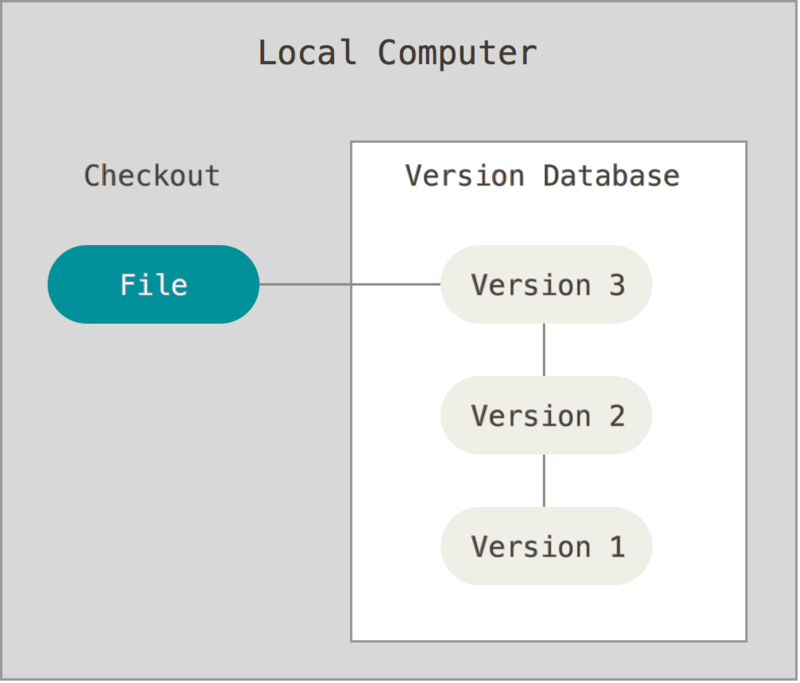
\includegraphics[scale=0.25]{Gambar/localvcs.png}
	\caption{Local version control}
	\label{fig:localvcs}
\end{figure}

Gambar \ref{fig:localvcs} merupakan struktur dari \textit{Local Version Control Systems}. \textit{Database local Version Control Systems} ini tersimpan pada \textit{local} direktori di komputer. \textit{Database} ini menyimpan perubahan \textit{file} ke dalam beberapa versi atau \textit{state}.\textit{Local Version Control}, dapat melakukan \textit{checkout} \textit{file} ke versi atau \textit{state} tertentu.   
 
\subsubsection{Centralized Version Control Systems}
\begin{figure}[H]
	\centering
		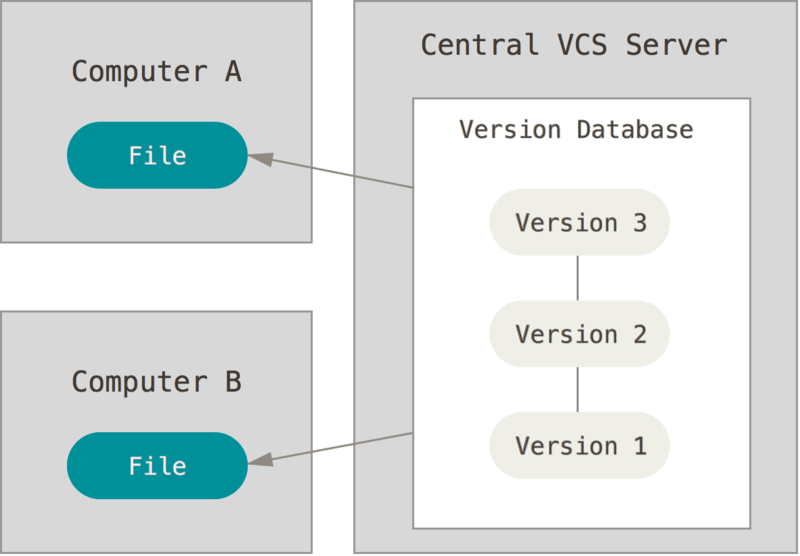
\includegraphics[scale=0.25]{Gambar/centralizedvcs.png}
	\caption{Centralized version control}
	\label{fig:cvcs}
\end{figure}

\textit{Local Version Control} hanya menyimpan \textit{file} pada satu komputer saja. Muncul masalah baru ketika \textit{user} ingin berkolaborasi dengan \textit{user} lain. Untuk mengatasi masalah ini dikembangkan \textit{Centralized version control}. Gambar \ref{fig:cvcs} merupakan struktur dari \textit{Centralized Version Control Systems}. Dalam \textit{Centralized Control Version Systems} terdapat sebuah \textit{server} yang menyimpan setiap versi \textit{file}, dan klien yang dapat melakukan \textit{checkout} \textit{file}\cite{chacon2014pro}.

Sistem \textit{Centralized Version Control Systems} memiliki beberapa kelebihan. Setiap \textit{user}  dapat mengetahui pekerjaan yang dilakukan oleh \textit{user} lain. Administrator dapat lebih mudah mengontrol \textit{database} \textit{Centralized Version Control Systems} dibandingkan dengan \textit{database} \textit{Local Version Control Systems} dari setiap klien.      

Tetapi, \textit{Centralized Version Control Systems} juga memiliki kelemahan. Jika \textit{server} pusat \textit{Centralized Version Control Systems} mati , maka perubahan pada \textit{file} tidak bisa disimpan. Klien juga tidak dapat melakukan kolaborasi dengan klien lain. Jika \textit{harddisk} pada server rusak, maka semua versi \textit{file} akan hilang.  

\subsubsection{Distributed Version Control Systems}
\begin{figure}[H]
	\centering
		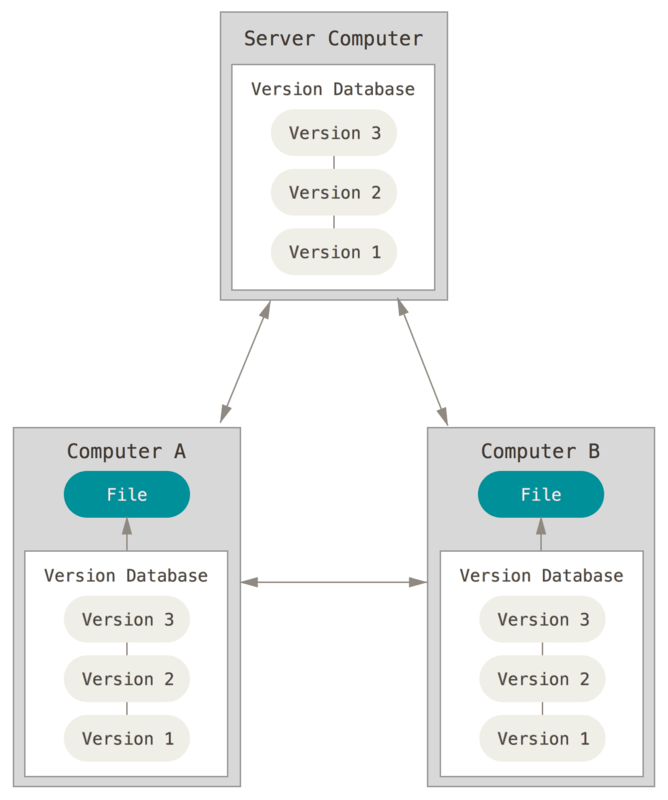
\includegraphics[scale=0.5]{Gambar/dvcs.png}
	\caption{Distributed version control}
	\label{fig:dvcs}
\end{figure}
Gambar \ref{fig:dvcs} merupakan struktur dari \textit{Distributed Version Control Systems}. Dalam sebuah DVCS (seperti Git, Mercurial, Bazaar atau Darcs), klien tidak hanya melakukan \textit{checkout} untuk \textit{snapshot} terakhir setiap \textit{file}, namun klien juga memiliki salinan dari repositori tersebut\cite{chacon2014pro}. Dengan kata lain setiap klien memiliki \textit{version database local} pada komputernya. Jika server pusat mati, klien masih bisa melakukan kolaborasi dan klien manapun dapat mengirimkan kembali salinan repositori ke \textit{server}.

\subsection{Cara Kerja Git}
Salah satu perbedaan antara Git dengan VCS lainnya adalah dalam cara Git memperlakukan datanya\cite{chacon2014pro}. Kebanyakan sistem \textit{Version Control Systems} lain menyimpan informasi sebagai daftar perubahan \textit{file}. Pada gambar \ref{fig:deltas}, terdapat tiga \textit{file}.\textit{Version Control Systems} menyimpan \textit{file} A, B, dan C pada versi pertama saja. Untuk versi kedua dan seterusnya yang disimpan adalah perubahan pada setiap \textit{file}. Sistem ini disebut juga sebagai \textit{delta-based Version Control Systems}. 
\begin{figure}[H]
	\centering
		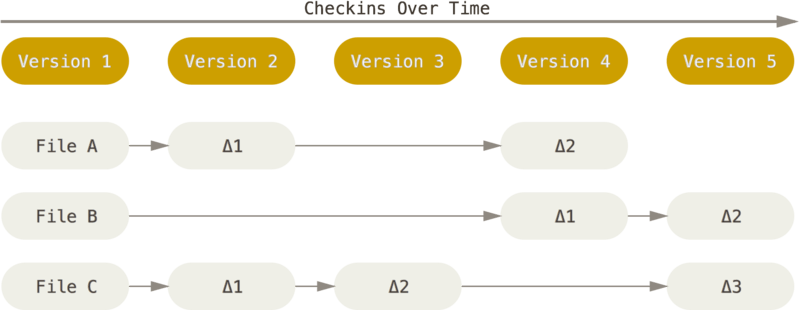
\includegraphics[scale=0.5]{Gambar/deltas.png}
	\caption{Menyimpan data sebagai \textit{snapshots} dari \textit{project}}
	\label{fig:deltas}
\end{figure}


Berbeda dengan \textit{Version Control Systems} lainnya, Git memperlakukan datanya sebagai sebuah kumpulan \textit{snapshot} dari sebuah miniatur \textit{file system}\cite{chacon2014pro}. Setiap kali dilakukan \textit{commit}, git merekam \textit{state} dari sekumpulan \textit{file} dan menyimpanannya sebagai \textit{reference} \textit{snapshot} tersebut. Jika ada \.Gambar \ref{fig:snapshots}, menunjukkan \textit{snapshots} dari \textit{file} A, B, dan C. Pada versi dua \textit{file} B tidak mengalami perubahan, sehingga \textit{file} yang disimpan adalah referensi \textit{file} B pada versi sebelumnya.
\begin{figure}[H]
	\centering
		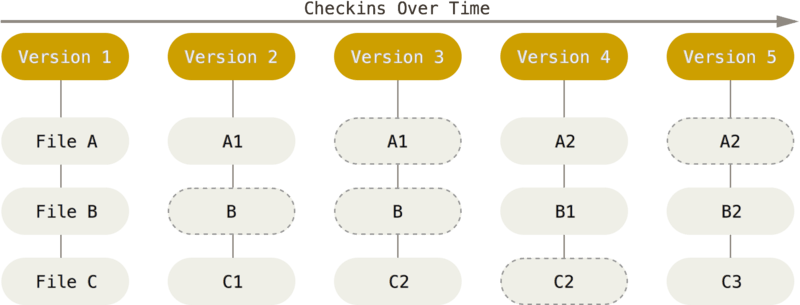
\includegraphics[scale=0.5]{Gambar/snapshots.png}
	\caption{Menyimpan data sebagai perubahan terhadap versi dasar dari setiap \textit{file}}
	\label{fig:snapshots}
\end{figure}

\subsubsection{State pada Git}
Terdapat tiga \textit{state} pada Git yaitu \textit{committed}, \textit{modified}, and \textit{staged}\cite{chacon2014pro}.\textit{Committed} adalah \textit{state} dimana data sudah disimpan di \textit{local database}. \textit{Modified} \textit{state} dimana terdapat perubahan pada \textit{file}, namun \textit{file} tersebut belum di \textit{commit} ke \textit{database}. \textit{Staged} adalah \textit{state} dimana \textit{file} telah ditandai untuk kemudian dilakukan commit.

Terdapat tiga bagian utama dari sebuah \textit{project} Git yaitu direktori Git, direktori kerja, dan staging area\cite{chacon2014pro}. Direktori Git merupakan tempat dimana Git menyimpan \textit{metadata} dan \textit{object database} dari \textit{project}. \textit{Working ree} adalah suatu \textit{snapshot} dari \textit{project}. Sekumpulan \textit{file} ini diambil dari \textit{database} di direktori Git dan ditempatkan pada \textit{disk} untuk digunakan dan dimodifikasi. \textit{Staging} area adalah \textit{file} yang menyimpan informasi mengenai apa yang menjadi \textit{commit} selanjutnya. \textit{File staging area} terdapat pada direktori Git. Untuk lebih jelasnya, lihat gambar \ref{fig:git_state}.

Alur kerja dari Git adalah sebagai berikut:
\begin{enumerate}
\item Melakukan modifikasi pada \textit{file}
\item Menandai perubahan pada \textit{file} dan memindahkannya ke \textit{staging area}.
\item Mengambil \textit{file} dari \textit{staging area} dan menyimpan \textit{snapshot} ke direktori Git. Proses ini disebut dengan \textit{commit}.
\end{enumerate}  

\begin{figure}[H]
	\centering
		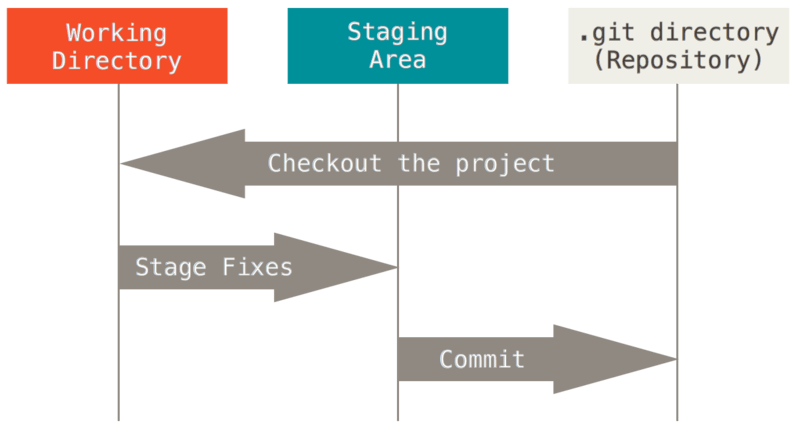
\includegraphics[scale=0.5]{Gambar/git_state.png}
	\caption{ \textit{Working tree}, \textit{Staging area}, dan Git direktori}
	\label{fig:git_state}
\end{figure}

\subsection{Operasi Dasar pada Git}
Pada subbab ini dijelaskan mengenai operasi dasar dalam Git dan sintaks-sintaksnya.
Berikut ini adalah operasi-operasi dasar dalam Git:
\begin{enumerate}
\item Init\\
\$ git init [project-name]\\
Operasi digunakan untuk membuat repositori local baru dengan nama tertentu. Bisa juga digunakan untuk merekam direktori yang sudah ada.
\item Add\\
\$ git add [file]\\
Operasi ini digunakan untuk menandai perubahan pada \textit{file} dan memindahkan \textit{file} tersebut ke \textit{staging area}. 
\item Commit\\
\$ git commit -m "[descriptive message]" \\
Operasi digunakan untuk merekam \textit{snapshot} pada \textit{file}. Dengan kata lain 

\item Clone
\item Fetch
\item Merge
\item Merge
\item Pull
\item Push
\item Checkout
\item Branch
\item Diff
\end{enumerate}

\subsection{Git Checkout}

\section{JGit}
\subsection{Porcelain API}
\subsection{Plumbing API}

\section{Selenium WebDriver}
\section{Apache Commons CLI}
